\documentclass[11pt,a4paper]{article}
\usepackage[utf8]{inputenc}
\usepackage[T1]{fontenc}
\usepackage[provide=*]{babel}
\babelprovide[main,import]{french}
\IfFileExists{lmodern.sty}{\usepackage{lmodern}}{}
\usepackage[a4paper,margin=2.5cm]{geometry}
\usepackage{setspace}
\onehalfspacing
\usepackage{amsmath}
\usepackage{array}
\usepackage{microtype}
\usepackage{graphicx}
% Les images (logos AMU/AMSE, signature) vivent dans Memoire/logos/.
\graphicspath{{../logos/}{logos/}{./}}
\usepackage{xcolor}
\usepackage{fancyhdr}
\IfFileExists{xurl.sty}{\usepackage{xurl}}{}
\usepackage[hidelinks]{hyperref}
\usepackage{ragged2e}\hypersetup{colorlinks=true, linkcolor=black, urlcolor=blue!50!black, citecolor=black}
\IfFileExists{float.sty}{\usepackage{float}}{}
\IfFileExists{booktabs.sty}{\usepackage{booktabs}}{}
\IfFileExists{tabularx.sty}{\usepackage{tabularx}}{}
\IfFileExists{tikz.sty}{\usepackage{tikz}\usetikzlibrary{arrows.meta,positioning}}{}
\definecolor{myblue}{RGB}{35,55,120}
\definecolor{mygreen}{RGB}{42,120,80}
\definecolor{myred}{RGB}{145,55,55}
\definecolor{mygray}{RGB}{85,85,85}
\IfFileExists{titlesec.sty}{%
  \usepackage{titlesec}%
  \titleformat{\section}{\large\bfseries\color{myblue}}{\thesection.}{0.5em}{}%
  \titleformat{\subsection}{\normalsize\bfseries\color{myblue!85}}{\thesubsection.}{0.5em}{}%
  \titlespacing*{\section}{0pt}{1.2\baselineskip}{0.6\baselineskip}%
  \titlespacing*{\subsection}{0pt}{1.0\baselineskip}{0.45\baselineskip}%
  \titlespacing*{\subsubsection}{0pt}{0.8\baselineskip}{0.35\baselineskip}%
}{}
\pagestyle{fancy}\fancyhf{}
\fancyhead[L]{\footnotesize Rapport de stage, M2 Econometrics \& Statistics}
\fancyhead[R]{\footnotesize J.D'OLIVEIRA}
\fancyfoot[C]{\thepage}
\setlength{\headheight}{14pt}

% Repli si une image n'est pas encore fournie (logos AMU/AMSE, signature).
% Des que le .png est depose dans ce dossier, il est utilise automatiquement.
\newcommand{\imgOrPlaceholder}[3]{%
  \IfFileExists{../logos/#2}{\includegraphics[#1]{../logos/#2}}{%
   \IfFileExists{logos/#2}{\includegraphics[#1]{logos/#2}}{%
    \IfFileExists{#2}{\includegraphics[#1]{#2}}{%
     \fbox{\parbox[c][1.4cm][c]{4.2cm}{\centering\scriptsize\color{red}\textbf{#3}\\[1mm]fichier \texttt{#2} absent}}}}}%
}

\newcommand{\rapportdate}{22 août 2026}
% Comptes issus des métadonnées du package, régénérés par
% code/package_metadata/export_report_eligibility_counts.py.
% Fichier genere par code/package_metadata/export_report_eligibility_counts.py.
\newcommand{\BostonEligibleCount}{17}
\newcommand{\DiabetesEligibleCount}{11}
\newcommand{\DragonflyEligibleCount}{0}
\newcommand{\FloridaEligibleCount}{0}
\newcommand{\SeshatEligibleCount}{13}
\newcommand{\AirbnbEligibleCount}{2}


\begin{document}
\hypersetup{pageanchor=false}
\pagenumbering{gobble}

% ============================ PAGE DE TITRE ============================
\begin{titlepage}
\centering
\vspace*{1.5cm}
{\scriptsize AIX-MARSEILLE UNIVERSITÉ, AIX-MARSEILLE SCHOOL OF ECONOMICS\par}
{\scriptsize Master Econometrics \& Statistics, M2 Econometrics, Data Science (EDS)\par}
\vspace{2cm}
{\color{myblue}\rule{\textwidth}{1.2pt}}\\[0.6cm]
{\LARGE\bfseries Constitution d'une banque de données de référence pour la validation de modèles prédictifs spatio-temporels\par}
\vspace{0.4cm}
{\large\itshape D'un système de métadonnées enrichies à un banc d'essai exécutable\par}
{\color{myblue}\rule{\textwidth}{1.2pt}}\\[1.2cm]

{\large\textbf{Johnny D'OLIVEIRA}\par}
\vspace{1.5cm}
\begin{tabular}{>{\bfseries}p{4.9cm}p{8.9cm}}
Organisme d'accueil & INRAE, Centre d'Avignon, unité Écodéveloppement \\[0.2cm]
Encadrant professionnel & Ghislain Geniaux, chargé de recherche à l'INRAE \\[0.2cm]
Encadrement académique & Badih GHATTAS et Pierre Michel, responsables du parcours EDS, AMSE \\[0.2cm]
Période & Avril à septembre 2026 \\
\end{tabular}
\vfill
{\footnotesize Rapport de stage de fin d'études, \rapportdate\par}
\end{titlepage}

% ============================ PAGE NON-PLAGIAT ============================
\thispagestyle{empty}
% Logos
\noindent
\begin{minipage}{0.45\textwidth}
    \imgOrPlaceholder{height=1.5cm}{logo_amu.png}{LOGO AMU}
\end{minipage}
\hfill
\begin{minipage}{0.45\textwidth}
    \raggedleft
    \imgOrPlaceholder{height=1.5cm}{logo_amse.png}{LOGO AMSE}
\end{minipage}

\vspace{3.5cm}

\begin{center}
    \textbf{\Large ENGAGEMENT DE NON-PLAGIAT}
\end{center}

\vspace{3cm}

\noindent
Je soussigné, \textit{Johnny D'OLIVEIRA},
déclare être pleinement conscient que le plagiat, consistant à copier des documents ou une partie d'un document publié sous quelque forme que ce soit et sur quelque support que ce soit, y compris les publications en ligne, constitue une violation du droit d'auteur et des droits voisins, ainsi qu'une fraude pure et simple.

\vspace{0.5cm}

\noindent
En conséquence, je m'engage par la présente à citer toutes les sources et tous les auteurs auxquels j'ai eu recours pour rédiger mon rapport de stage et ses annexes.

\vspace{2cm}

\noindent
\begin{minipage}[t]{0.45\textwidth}
Date : \rapportdate
\end{minipage}
\hfill
\begin{minipage}[t]{0.45\textwidth}
\raggedleft
\begin{minipage}[t]{3.5cm}
\centering
Signature:

\vspace{0.2cm}

\imgOrPlaceholder{width=2.5cm}{signature.png}{SIGNATURE}\\[-0.1cm]
Johnny D'OLIVEIRA
\end{minipage}
\end{minipage}

\newpage

% ============================ TABLE DES MATIERES ============================
\thispagestyle{empty}
\tableofcontents
\newpage
\hypersetup{pageanchor=true}
\pagenumbering{arabic}

% ============================ INTRODUCTION ============================
\section{Introduction}

Ce rapport rend compte du stage de fin d'études réalisé au sein de l'unité Écodéveloppement de l'INRAE, au centre d'Avignon. Il présente la mission qui m'a été confiée et en propose une lecture analytique à partir des compétences acquises durant le Master. La problématique de départ est méthodologique. Il s'agit de déterminer comment valider de manière crédible des méthodes statistiques destinées aux données spatiales et spatio-temporelles lorsque les jeux de données de référence disponibles restent peu nombreux, dispersés et difficilement comparables.

La validation d'une méthode prédictive peut emprunter trois voies complémentaires. La première consiste à établir mathématiquement ses propriétés, notamment asymptotiques. Une telle démonstration n'est toutefois pas toujours accessible pour des estimateurs complexes. La deuxième repose sur des simulations de Monte-Carlo. Comme le processus générateur des données est connu, celles-ci permettent d'évaluer la qualité de l'inférence sur les paramètres et la capacité prédictive du modèle. Elles occupent ainsi une place importante dans l'évaluation des méthodes statistiques.

 Les simulations présentent néanmoins une limite importante. Elles ne peuvent couvrir qu'un nombre restreint de configurations, alors que les données spatiales et spatio-temporelles peuvent combiner des distributions non normales, des corrélations entre variables, des non-linéarités, des interactions ou encore des erreurs de mesure. Aucun plan de simulation ne peut reproduire toute cette diversité. Une troisième voie consiste donc à confronter les méthodes à des cas empiriques variés. Elle permet d'observer leur comportement dans des situations qui n'ont pas été entièrement construites par l'expérimentateur.


Cette approche possède elle aussi ses limites. Dans les cas empiriques, les véritables paramètres du processus générateur sont inconnus. Il devient alors possible d'évaluer la capacité prédictive d'un modèle, mais beaucoup plus difficile de juger directement la qualité de l'inférence sur ses paramètres. Une banque de données réelles ne remplace donc pas les expériences de Monte-Carlo. Elle constitue une couche de validation complémentaire. Cette distinction est particulièrement importante pour les méthodes d'apprentissage automatique, puisqu'un modèle peut fournir de bonnes prédictions sans nécessairement permettre une interprétation correcte des effets des variables, notamment en présence d'endogénéité.


C'est dans cette troisième voie qu'apparaît une difficulté structurelle. De nombreux jeux de données réels existent, mais ils sont rarement disponibles sous une forme homogène. Leur documentation ne permet pas toujours de retrouver facilement la variable réponse, les covariables, la structure spatiale ou la spécification utilisée dans la publication d'origine. Ils sont également dispersés entre publications scientifiques, packages statistiques et entrepôts de données. Cette difficulté n'est pas propre aux méthodes spatiales. En apprentissage automatique, des initiatives telles que PMLB ont cherché à regrouper et standardiser des jeux de données afin de faciliter l'évaluation comparative des méthodes (Olson \textit{et al.}, 2017). Plus généralement, la littérature sur le benchmarking des méthodes computationnelles souligne l'importance de disposer de protocoles et de ressources partagés pour rendre les comparaisons plus transparentes et reproductibles (Weber \textit{et al.}, 2019 ; Thiyagalingam \textit{et al.}, 2022).


Les données spatiales ajoutent une difficulté supplémentaire. Les observations proches géographiquement peuvent être dépendantes, ce qui remet en cause certains protocoles classiques d'évaluation fondés sur l'indépendance entre les échantillons d'entraînement et de test. La constitution d'une banque de référence dans ce domaine suppose donc non seulement de rassembler des jeux de données, mais aussi de documenter suffisamment leur structure pour permettre l'utilisation de protocoles de validation adaptés.

Le but de mon stage est de contribuer à la construction d'une telle banque de données de référence. Celle-ci est conçue comme un banc d'essai structuré plutôt que comme une simple accumulation de jeux disponibles. Le travail comprend également le développement d'une architecture logicielle permettant de documenter, préparer et exploiter ces données dans des conditions comparables.

Le rapport est organisé en trois parties principales. La première présente le contexte du stage, l'organisme d'accueil et l'écosystème scientifique dans lequel s'inscrit la mission. La deuxième décrit le travail réalisé, depuis la constitution et la documentation de la banque jusqu'au développement du dispositif permettant d'exécuter les benchmarks. Elle revient également sur les principales contraintes et sur les solutions mises en place. La conclusion propose enfin un bilan du travail accompli, de ses limites et des apports du Master dans sa réalisation.
% ============================ CONTEXTE ============================
\section{Contexte}

Cette section présente l'environnement scientifique et institutionnel dans lequel s'est déroulé le stage. Elle revient d'abord sur l'organisme et l'unité d'accueil, puis sur l'écosystème de science ouverte mobilisé au cours de la mission. Elle permet enfin de situer les principaux éléments qui ont facilité le travail ainsi que les contraintes auxquelles il a fallu répondre.

\subsection{L'organisme d'accueil}

L'INRAE, Institut national de recherche pour l'agriculture, l'alimentation et l'environnement, est un établissement public de recherche français issu de la fusion, en 2020, de l'INRA et d'IRSTEA. Ses activités portent sur les enjeux liés à l'agriculture, à l'alimentation et à l'environnement. Sa production repose principalement sur la création et la diffusion de connaissances scientifiques, notamment sous la forme de publications, de logiciels et de jeux de données. Dans ce contexte, la valeur d'un travail de recherche tient moins à une logique marchande qu'à la robustesse, à la reproductibilité et à la capacité de réutilisation des résultats produits.

Le stage s'est déroulé au sein de l'unité Écodéveloppement, rattachée au centre INRAE Provence-Alpes-Côte d'Azur et au département ACT, « Sciences pour l'action, les transitions, les territoires ». Ce département étudie notamment les transformations des socio-écosystèmes et des systèmes agroalimentaires, dans le but d'accompagner les transitions vers la durabilité et d'éclairer l'action publique.

Créée en 1983 autour du concept d'écodéveloppement, l'unité a progressivement élargi ses approches disciplinaires et ses objets de recherche. À partir des années 1990, elle a notamment accueilli des travaux en économie et en sociologie sur les politiques publiques agro-environnementales. L'analyse spatiale occupe également une place ancienne dans ses recherches. Dès les années 2000, certaines problématiques foncières ont été étudiées à l'aide de l'économétrie spatiale.

Aujourd'hui, les travaux de l'unité portent notamment sur la compréhension et l'accompagnement de l'écologisation des systèmes agroalimentaires, à différentes échelles allant des systèmes de production aux territoires. L'unité se caractérise par une forte interdisciplinarité. Elle réunit notamment des agronomes, des sociologues, des économistes, des géographes et des écologues, et mobilise aussi bien des méthodes qualitatives que des méthodes quantitatives telles que l'économétrie, la géomatique et l'analyse spatiale.

L'unité développe aussi des outils méthodologiques pour l'économétrie spatiale. C'est le cas du package R \texttt{mgwrsar}, qui permet d'estimer des modèles de régression tenant compte de la dépendance spatiale et de relations qui peuvent varier selon la structure géographique des données (Geniaux \& Martinetti, 2018).

Un autre développement récent est le package \texttt{spboost}, disponible sur le CRAN (Geniaux, 2026a). Il propose une approche par boosting pour des modèles spatiaux non linéaires, en lien avec des travaux menés sur le rapprochement entre économétrie spatiale et apprentissage statistique (Geniaux, 2023). Ces outils donnent un cadre concret au stage, car ils montrent le besoin de comparer plusieurs estimateurs spatiaux sur des jeux de données réels et bien documentés.

L'unité travaille aussi sur des modèles adaptés à d'autres types de réponses. C'est notamment le cas des modèles probit spatiaux, utilisés lorsque la variable à expliquer est binaire, par exemple oui/non ou présence/absence (Martinetti \& Geniaux, 2017). Cette perspective est importante pour la suite du projet, car plusieurs jeux de données repérés ne relèvent pas d'une régression continue classique.

Ces activités expliquent directement l'intérêt de la mission pour l'unité. Le développement d'une nouvelle méthode ne suffit pas à établir son comportement empirique. Il faut également pouvoir l'évaluer sur des configurations spatiales variées et le comparer à des méthodes existantes dans des conditions homogènes. La banque de données construite pendant le stage vise à fournir progressivement ce matériel commun d'évaluation.

\subsection{Un écosystème de recherche ouvert}

La mission repose aussi sur l'écosystème de la science ouverte. Les jeux de données mobilisés dans le projet ne proviennent pas d'une seule source. Certains sont diffusés dans des entrepôts comme Dryad, Zenodo, Figshare ou Dataverse. D'autres sont décrits dans la littérature, distribués dans des bibliothèques R ou Python, ou mis à disposition par des portails institutionnels comme l'INSEE et Eurostat.

Les dépôts et les infrastructures bibliographiques apportent plus que des fichiers. Ils fournissent des métadonnées, des identifiants pérennes, des liens vers les publications et des informations sur les licences. Ces éléments sont nécessaires pour conserver la trace de l'origine de chaque jeu de données et pour savoir dans quelles conditions il peut être réutilisé. Cette exigence rejoint les principes FAIR, qui recommandent que les données soient trouvables, accessibles, interopérables et réutilisables (Wilkinson \textit{et al.}, 2016).

Dans la pratique, l'information reste souvent incomplète ou dispersée. Un DOI peut renvoyer vers une page de dépôt sans fournir directement la formule utilisée dans l'article. Un article peut décrire les variables du modèle sans donner un fichier directement exploitable. Un package peut contenir un jeu de données utile sans référence bibliographique précise. Le travail de curation consiste alors à relier les sources entre elles, puis à documenter ce qui est confirmé, ce qui reste incertain et ce qui ne peut pas être utilisé.

La reproductibilité ne dépend donc pas seulement de la disponibilité des données. Elle suppose aussi de connaître les traitements appliqués, les variables retenues, la structure spatiale, les versions logicielles et les choix effectués pendant l'analyse. Plusieurs travaux sur la reproductibilité montrent que ces informations doivent être explicites pour permettre à d'autres chercheurs de reprendre une analyse dans de bonnes conditions (Konkol \textit{et al.}, 2019 ; Sandve \textit{et al.}, 2013).

Les principes de traçabilité ont directement guidé la construction de la banque. Les jeux recensés doivent être accompagnés d'éléments permettant d'identifier leur origine, de comprendre leur contenu et de décider s'ils peuvent être intégrés au benchmark. La finalité n'est donc pas seulement de stocker des données, mais de construire une ressource vérifiable et réutilisable.

Le projet a enfin une vocation de valorisation scientifique. Une première forme de diffusion prendra la forme d'un \textit{data paper} consacré à la banque et à son processus de construction. L'intégration dans l'écosystème R doit aussi permettre à d'autres utilisateurs de mobiliser les jeux documentés dans des protocoles d'évaluation reproductibles.


\subsection{Les conditions de réalisation de la mission}

L'expertise méthodologique de l'unité m'a permis de mieux cerner les éléments requis pour documenter un jeu de données spatial : variable réponse, covariables, structure géographique, formule de régression et familles d'estimateurs pertinentes. J'ai aussi pu m'appuyer sur les bibliothèques déjà développées ou utilisées par le labo, qui ont fourni des méthodes de référence et des premiers jeux de données pour tester le dispositif.

L'accès aux ressources scientifiques a constitué un autre appui. Les articles, les entrepôts de données et les métadonnées bibliographiques ont permis d'identifier de nombreux jeux candidats. L'accès institutionnel aux publications et les orientations de l'encadrant vers plusieurs articles clés ont facilité la vérification des variables, des modèles et des sources. La participation au colloque d'économétrie spatiale à Paris a aussi contribué à mieux situer le projet, notamment au croisement entre économétrie spatiale et apprentissage statistique.

Le travail a également été facilité par l'utilisation d'assistants IA, qui m'ont aidé à automatiser certaines tâches répétitives, comme l'exploration de fichiers, la génération de scripts, la structuration de fiches ou la synthèse de documents. Leur rôle est toutefois resté encadré : les informations extraites devaient être vérifiées dans les sources, et les formules ou variables non confirmées ne devaient pas être inventées.

Plusieurs contraintes ont marqué la mission. Les sources sont hétérogènes, les métadonnées souvent incomplètes et certains articles ne fournissent pas directement les fichiers nécessaires pour reproduire leur analyse. Les données demandent parfois un travail de préparation conséquent avant de pouvoir être utilisées dans un benchmark. Les scripts automatisent une partie des contrôles sur les licences, les DOI, les liens vers les publications et les fichiers locaux, mais les cas ambigus doivent encore être vérifiés manuellement.

La continuité du travail a aussi guidé l'organisation du dépôt. Les fichiers bruts, les scripts de transformation, les fiches de synthèse et les métadonnées destinées au package ont été séparés afin que le projet puisse être repris plus facilement. À mesure que le corpus s'est agrandi, cette organisation a aussi permis de réduire la dépendance à la mémoire de ces assistants et de rendre les décisions de curation plus traçables.

% ============================ MISSION ============================
\section{La mission}

La mission porte sur la constitution d'une banque de données spatiales et spatio-temporelles destinée à l'évaluation de méthodes prédictives. Sa réalisation a progressivement conduit à développer deux composantes complémentaires : des activités de collecte, de documentation et de curation des jeux de données, ainsi qu'une infrastructure qui les rend directement exploitables selon des règles communes de validation et de comparaison des estimateurs.

Cette section présente les objectifs, le périmètre et les choix méthodologiques du projet. Elle décrit ensuite le système de curation, son évolution au cours du stage et l'infrastructure développée pour transformer le catalogue en banc d'essai exécutable. Enfin, elle revient sur les principaux problèmes observés, l'état actuel du projet et les apports de ce travail pour l'unité.


\subsection{Objectif et périmètre}

La mission vise à construire une banque de jeux de données réels pour évaluer des méthodes prédictives spatiales. Il ne s'agit pas seulement de rassembler des fichiers, mais de produire une ressource documentée, vérifiable et directement exploitable dans des protocoles de comparaison reproductibles.

Les données spatiales peuvent réunir plusieurs difficultés simultanément : relations non linéaires, interactions entre variables, dépendance entre voisins et hétérogénéité selon les lieux. Dans une simulation Monte Carlo, le chercheur choisit lui-même le mécanisme qui génère les données, souvent appelé DGP pour \textit{data-generating process}. Si ce mécanisme ne représente qu'une seule difficulté, par exemple une dépendance de type SAR sans hétérogénéité ni non-linéarité, il favorise naturellement les méthodes conçues pour ce cas précis. Même en variant les simulations, il reste difficile de reproduire toutes les combinaisons rencontrées dans des cas empiriques.

Tester une méthode sur seulement quelques jeux réels, comme le font beaucoup d'articles, ne suffit pas toujours à apprécier sa robustesse. Un bon résultat peut dépendre fortement des jeux choisis. L'intérêt principal de la banque est donc de permettre l'évaluation d'un estimateur sur de nombreux jeux réels, documentés et variés. On peut alors observer si ses performances restent stables dans plusieurs contextes, et pas seulement dans une situation artificielle construite pour l'expérience.

Le travail s'organise autour de trois objectifs. D'abord, collecter et curer des jeux de données spatiaux issus de plusieurs sources. Ensuite, définir des schémas communs de séparation et d'évaluation. Enfin, comparer plusieurs familles d'estimateurs dans des conditions homogènes. Ces trois volets sont liés, mais ils n'ont pas encore le même niveau de maturité. Les pipelines de collecte et de documentation peuvent être relancés sur de nouvelles sources. La partie benchmark est déjà opérationnelle, mais seulement pour les jeux suffisamment préparés et validés.

Le périmètre a donc été construit progressivement. Une première phase a porté sur les jeux disponibles dans des packages R et Python. Ce choix permettait de partir de données déjà accessibles localement, avec une structure relativement stable. Le travail a ensuite été étendu aux jeux associés à une publication scientifique, notamment lorsqu'un dépôt de données, une formule de régression ou une liste de variables permettait d'envisager une réutilisation.

La priorité actuelle reste la régression spatiale sur données réelles, avec une variable réponse exploitable, des covariables identifiées et une structure géographique claire. Les jeux spatio-temporels, les panels, les réponses binaires ou les variables de comptage ne sont pas écartés définitivement, mais leur intégration demande des règles spécifiques. Ils sont donc conservés lorsqu'ils sont bien documentés, sans être automatiquement promus dans le benchmark principal.

La banque doit ainsi être comprise comme une ressource évolutive. Chaque dataset traverse une série d'étapes allant de la collecte à la promotion éventuelle au sein du package. Les filtres servent à distinguer les données directement utilisables, les candidats à compléter et les sources à écarter. Cette organisation permet d'étendre progressivement le catalogue tout en gardant une trace claire des décisions prises.

\subsection{Des métadonnées au choix méthodologique}

Un des choix structurants du projet a été de ne pas limiter les métadonnées à une fonction descriptive. Le système a été conçu pour rassembler les métadonnées attendues lors des étapes ultérieures de préparation, de validation et de modélisation. Une fiche ne doit donc pas seulement indiquer ce que contient un jeu de données. Elle doit également préciser dans quelles conditions celui-ci peut être utilisé pour un benchmark.

Cette logique repose sur une chaîne progressive. Les données sont d'abord associées à une couche de métadonnées enrichies décrivant leur provenance, leur structure et leur usage dans la littérature. Ces informations permettent ensuite de caractériser le jeu, d'identifier les familles d'estimateurs compatibles et de sélectionner les éléments nécessaires au pipeline d'analyse. Les décisions ne sont pas toutes produites automatiquement. Certaines informations sont extraites directement des sources, d'autres sont reconstruites lorsque la documentation le permet, puis vérifiées avant leur utilisation.

La couche de métadonnées est organisée autour de plusieurs dimensions complémentaires. Elle comprend la variable réponse, les covariables et la formule utilisée dans la publication lorsqu'elle est disponible. Elle conserve également les informations de provenance, notamment les DOI de la publication et du jeu de données, ainsi que la source et le mode de récupération. D'autres champs décrivent la structure spatiale ou spatio-temporelle, le nombre d'unités et de périodes, le type de variable réponse, la résolution spatiale et l'étendue temporelle. Enfin, des informations relatives au code disponible, à la licence et à la reproductibilité complètent la fiche.

Cette structuration permet de distinguer des jeux qui seraient difficilement comparables à partir de leur seul format informatique. Deux fichiers peuvent, par exemple, contenir le même nombre de colonnes et d'observations tout en correspondant à des situations méthodologiques très différentes selon qu'ils décrivent une coupe transversale spatiale, un panel, une variable réponse continue ou un comptage. Les métadonnées servent ainsi à positionner chaque dataset dans un espace de caractéristiques qui pourra ensuite guider la sélection des estimateurs et des protocoles de validation pertinents.

L'intérêt de cette organisation apparaît au moment de l'exécution. Lorsqu'un jeu est suffisamment documenté, le package peut récupérer directement une partie des informations nécessaires au benchmark, notamment la variable réponse, les covariables, la formule et les informations spatiales disponibles. Cette normalisation réduit les traitements spécifiques aux jeux recensés et limite la nécessité de reconstituer manuellement leur configuration à chaque nouvelle analyse. Elle permet ainsi de relier la documentation de la banque à son utilisation effective au sein du package.
\newpage
\begin{table}[h]
\centering
\small
\begin{tabularx}{\textwidth}{>{\bfseries}p{4.1cm} X}
\toprule
Bloc & Informations principales \\
\midrule
Formule et variables &
Variable réponse, covariables, formule publiée ou reconstruite \\

Provenance &
DOI du jeu, DOI de la publication, source et mode de récupération \\

Caractéristiques du modèle &
Nature de la tâche, familles d'estimateurs compatibles et variantes \\

Structure des données &
Support spatial ou spatio-temporel, structure de panel, type de réponse et profil $N/T$ \\

Résolution et étendue &
Unité spatiale, emprise géographique et période couverte \\

Reproductibilité &
Disponibilité du code, dépôt source, licence et informations de réutilisation \\
\bottomrule
\end{tabularx}

\caption{Principaux blocs de métadonnées de la banque.}
\label{tab:metadata-blocks}
\end{table}
\begin{figure}[h]
\centering
\begin{tikzpicture}[
    node distance=0.55cm and 0.6cm,
    box/.style={rectangle, rounded corners, draw=myblue, fill=blue!5,
                text width=2.05cm, align=center, minimum height=1cm, font=\footnotesize},
    arr/.style={-{Stealth[length=2.5mm]}, myblue, thick}]
\node[box] (a) {Données};
\node[box, right=of a] (b) {Métadonnées};
\node[box, right=of b] (c) {Caracté-\\risation};
\node[box, right=of c] (d) {Estimateurs compatibles};
\node[box, right=of d] (e) {Benchmark};
\draw[arr] (a)--(b);
\draw[arr] (b)--(c);
\draw[arr] (c)--(d);
\draw[arr] (d)--(e);
\end{tikzpicture}
\caption{Des données documentées à leur utilisation dans le benchmark.}

\label{fig:chaine-methodologique}
\end{figure}


\subsection{Le système de curation}
La constitution d'une banque de données de cette ampleur suppose de rechercher, examiner et relier un grand nombre de sources hétérogènes. Réaliser toutes ces opérations entièrement à la main serait difficile à envisager. Le projet repose donc sur une chaîne de curation assistée par des agents IA, qui automatisent certaines tâches répétitives tout en maintenant une vérification humaine lorsque l'information engage la validité scientifique des fiches.

\subsubsection{Collecte et structuration des sources}

La collecte a été organisée autour de trois blocs de sources. Le bloc 1 regroupe les jeux de données distribués dans des packages R et Python, par exemple \texttt{spData}, \texttt{sf}, \texttt{GWmodel}, \texttt{gstat} ou \texttt{libpysal}. C'est l'entrée la plus stable, car les objets sont déjà accessibles et peuvent être inspectés localement.

Le bloc 2 est constitué des jeux associés à des publications scientifiques et déposés dans des entrepôts comme DataCite, Dryad, Zenodo, Figshare ou Dataverse. Le pipeline \texttt{run\_datacite\_harvest\_pipeline.py} automatise une partie de cette recherche. Il combine des mots-clés liés aux méthodes spatiales, des indices de géométrie, des filtres sur la taille des fichiers, les citations et les relations avec les articles. Les candidats retenus sont ensuite enrichis avec des informations issues de services comme OpenAlex ou Crossref lorsque celles-ci sont disponibles.

Le bloc 3 part directement des articles scientifiques publiés. Il consiste à récupérer les PDF accessibles, puis à chercher dans les sections empiriques ou dans les déclarations de disponibilité des données les DOI et les dépôts des jeux utilisés par les auteurs. Il complète le bloc 2 lorsque le papier décrit une application intéressante, mais que le jeu de données n'est pas repéré directement par les métadonnées des dépôts.

Les candidats issus de ces trois blocs rejoignent ensuite une même chaîne de traitement. Les données et les papiers associés sont récupérés lorsqu'ils sont accessibles légalement. Les informations nécessaires à leur documentation sont extraites, contrôlées, puis utilisées pour décider si le jeu peut continuer dans le pipeline. Certains candidats deviennent des jeux préparés pour le benchmark, d'autres restent en vérification manuelle ou sont écartés lorsqu'une information essentielle manque.


\subsubsection{Organisation et gestion des connaissances}

L'augmentation du nombre de jeux de données et de publications a progressivement rendu la gestion du corpus plus complexe. Dans la première organisation, l'assistant devait souvent relire les mêmes documents pour retrouver une information nécessaire à une nouvelle tâche. Cette méthode mobilisait une part croissante du contexte disponible. Or, la présence d'une information dans un contexte long ne garantit pas qu'elle soit utilisée de manière robuste par un modèle de langage (Liu \textit{et al.}, 2024).

Pour répondre à cette difficulté, la première version de l'infrastructure s'est appuyée sur l'implémentation open source proposée par Balu Kosuri (2026), elle-même fondée sur le modèle de \textit{LLM Wiki} décrit par Karpathy (2026). Cette approche ne correspond pas à un logiciel unique, mais à un principe d'organisation. Les sources brutes sont conservées, tandis que l'assistant construit progressivement des pages de synthèse reliées entre elles. Lorsqu'une nouvelle source est intégrée, elle peut compléter une fiche existante, créer de nouveaux liens ou conduire à réviser une synthèse. Le wiki constitue ainsi une mémoire cumulative, consultable et enrichie au fil du travail.

Le projet a ensuite adapté cette organisation aux besoins d'une banque de données destinée au benchmark spatial. Les publications sont d'abord organisées dans une bibliographie structurée avec JabRef. Lorsqu'un PDF est disponible, GROBID le convertit au format TEI afin de faciliter la consultation de son contenu. Les documents d'origine et les fichiers de données restent séparés des pages de synthèse, ce qui permet de revenir à la source lors d'une vérification.

Le wiki fournit une représentation lisible du corpus. Il est complété par un graphe de connaissances qui relie les jeux de données, les publications, les packages, les modèles et leurs principales caractéristiques. Lors d'une requête, le graphe permet d'abord d'identifier les ressources pertinentes. Le wiki fournit ensuite une synthèse lisible et contrôlable. Ce parcours évite de mobiliser tout le corpus pour chaque tâche et permet de construire un contexte plus ciblé.

Cette organisation ne remplace pas la validation scientifique. Des contrôles vérifient la structure des fiches et la cohérence de leurs informations. Les graphes de connaissances facilitent ainsi l'exploration d'informations hétérogènes tout en conservant un lien explicite avec les sources d'origine (Hogan \textit{et al.}, 2021).


\subsubsection{Validation et préparation des jeux de données}


L'automatisation de la collecte nécessite plusieurs niveaux de contrôle. Des vérifications déterministes examinent la structure des fiches et leur cohérence interne, par exemple lorsqu'une formule fait référence à une variable absente. Un modèle de langage peut également signaler certaines incohérences, mais cette évaluation reste une aide à la vérification, les modèles utilisés comme juges pouvant eux-mêmes présenter des biais (Zheng \textit{et al.}, 2023). Pour les jeux issus de publications scientifiques, les informations essentielles sont donc confrontées au papier source avant validation.

La préparation comprend aussi une harmonisation du support spatial. Les jeux peuvent être représentés sous forme de points, de polygones, de lignes ou de grilles, alors que plusieurs méthodes du benchmark nécessitent des coordonnées ponctuelles. Le script \texttt{build\_sf\_datasets.R} construit une représentation commune : les grilles sont représentées par leur centroïde, tandis que les polygones et les lignes sont ramenés à un point situé sur leur surface. La géométrie d'origine reste conservée.

La promotion vers le package dépend donc du niveau de preuve disponible. Pour les jeux issus de publications scientifiques, la variable réponse, les covariables, la formule ou la spécification empirique doivent être reliées au papier source. Pour les jeux issus de packages R ou Python, la justification peut provenir de la documentation du package, d'une vignette ou d'une publication associée. Dans tous les cas, le support spatial doit être suffisamment documenté pour permettre son utilisation dans le benchmark.

\subsection{Le package \texttt{spatialtidymodels}}

La constitution d'une banque de données ne suffit pas à elle seule à former un banc d'essai. Il faut également disposer d'un environnement capable d'appliquer plusieurs méthodes sur les mêmes jeux, selon des protocoles de validation communs, puis de restituer leurs performances dans un format homogène. Cette seconde composante du projet a conduit au développement du package R \texttt{spatialtidymodels}.

\subsubsection{Architecture et intégration des estimateurs}

\texttt{spatialtidymodels} est une extension en développement de l'écosystème \texttt{tidymodels}. Le package ne remplace pas les packages d'origine. Il fournit une interface commune pour appliquer leurs estimateurs aux mêmes jeux de données, avec les mêmes schémas d'évaluation, les mêmes métriques et des sorties comparables.

Plusieurs briques de \texttt{tidymodels} jouent un rôle particulier dans cette organisation. \texttt{parsnip} permet de définir un modèle sans fixer immédiatement tous les détails du moteur de calcul. \texttt{workflows} regroupe la formule, les éventuelles étapes de préparation et le modèle dans un même objet ajustable. \texttt{tune} s'occupe du réglage des hyperparamètres lorsque plusieurs valeurs doivent être testées, par exemple un nombre de voisins, un \textit{bandwidth}, un nombre d'arbres ou un nombre d'itérations de boosting.

L'intégration des estimateurs suit différentes logiques à travers les situations suivantes :

\begin{itemize}
    \item \textbf{Modèles déjà disponibles dans \texttt{tidymodels}.}
    Les forêts aléatoires, XGBoost ou MARS peuvent être appelés à travers des spécifications \texttt{parsnip}. Le travail consiste alors surtout à les inscrire dans le benchmark et à homogénéiser leurs sorties.

    \item \textbf{Modèles standards auxquels une information spatiale est ajoutée.}
    Certaines variantes reçoivent les coordonnées comme covariables, comme \texttt{random\_forest\_xy}, \texttt{xgboost\_xy} ou \texttt{earth\_xy}. Le cas \texttt{gam\_spatial} ajoute plutôt un lisseur spatial \texttt{s(x, y)} avec \texttt{mgcv::gam()}.

    \item \textbf{Méthodes spatiales reliées par une interface dédiée.}
    Des adaptateurs ou spécifications \texttt{parsnip} ont été développés pour relier \texttt{spatialreg}, \texttt{mgwrsar}, \texttt{spboost} et \texttt{spmoran} au moteur de benchmark. Ils transmettent les objets spatiaux nécessaires, comme les coordonnées, la matrice de poids $W$, le nombre de voisins ou le \textit{bandwidth}.

    \item \textbf{Méthodes nécessitant des objets spatiaux supplémentaires.}
    Certaines méthodes ne peuvent pas être ajustées avec la seule formule $Y \sim X$. Les modèles SAR, SEM et SDM utilisent une matrice de voisinage $W$, les méthodes GWR et MGWR utilisent un \textit{bandwidth}, tandis que d'autres approches exploitent des coordonnées, des distances ou des filtres spatiaux.
\end{itemize}

Cette organisation évite de présenter toutes les méthodes comme si elles avaient été réécrites dans le package. Pour certaines, le projet utilise les outils déjà disponibles. Pour d'autres, il ajoute une préparation spatiale des données. Pour les méthodes les plus spécifiques, il construit une couche d'adaptation afin de les faire entrer dans le même cadre de comparaison.

Le registre des estimateurs garde la trace de cette organisation. Il indique pour chaque méthode le backend utilisé, la famille d'estimateurs, les objets spatiaux nécessaires, les hyperparamètres réglables et les jeux de données compatibles. Il distingue aussi les paramètres estimés par le modèle, comme $\rho$ ou $\lambda$, des hyperparamètres qui peuvent être fixés par l'utilisateur ou optimisés par le benchmark lorsque \texttt{tune} est activé, comme un nombre de voisins, un \textit{bandwidth}, un nombre d'arbres ou un nombre d'itérations de boosting. Cette structure facilite l'ajout progressif de nouveaux estimateurs sans modifier toute l'architecture du benchmark.


\subsubsection{Quelques familles d'estimateurs intégrées}

Les estimateurs du registre ne sont pas seulement distingués par leur implémentation informatique. Ils répondent à plusieurs problématiques statistiques liées aux données géographiques. Dans le périmètre actuel du benchmark, ces méthodes sont principalement mobilisées pour des régressions en coupe transversale avec une variable réponse continue. Les réponses binaires, les comptages, les données de panel et les modèles spatio-temporels sont conservés comme extensions prévues, car ils exigent des spécifications et des protocoles d'évaluation propres.

\paragraph{Dépendance et hétérogénéité spatiales.}

Les données spatiales présentent deux propriétés majeures. La première est la dépendance spatiale, qui correspond à l'absence d'indépendance entre observations géographiquement proches. Le prix d'un logement, un niveau de pollution ou un rendement agricole peut ainsi dépendre de ce qui est observé dans les unités voisines. La seconde est l'hétérogénéité spatiale. Dans ce cas, la relation entre la variable réponse et les covariables n'est pas nécessairement identique sur tout le territoire. Une même covariable peut, par exemple, avoir un effet différent dans une zone urbaine dense, dans un espace rural ou dans une région montagneuse. Le Gallo distingue notamment l'hétéroscédasticité, les régimes spatiaux et l'instabilité continue des coefficients comme différentes manifestations de cette hétérogénéité (Le Gallo, 2002 ; Le Gallo, 2004).

Ces deux phénomènes doivent être diagnostiqués ensemble, sans être confondus. Une relation qui varie selon les lieux, mais qui est estimée comme une relation globale unique, peut produire des résidus regroupés dans l'espace. L'autocorrélation résiduelle observée peut alors traduire une dépendance spatiale, une hétérogénéité omise ou leur combinaison. Le choix d'un estimateur doit donc s'appuyer sur les diagnostics, la connaissance du phénomène étudié et l'objectif prédictif retenu.

\paragraph{Références globales et modèles prédictifs.}

La régression linéaire ordinaire constitue la référence la plus simple :

\begin{equation}
    \mathbf{y}=X\boldsymbol{\beta}+\boldsymbol{\varepsilon}.
\end{equation}

Elle suppose qu'un même vecteur de coefficients $\boldsymbol{\beta}$ s'applique à toutes les observations. Les GAM, MARS, Random Forest et XGBoost complètent cette référence en autorisant des relations non linéaires ou des interactions entre covariables. Ils sont indispensables au benchmark, car ils permettent d'établir si une structure spatiale explicite apporte un gain réel par rapport à un modèle global ou prédictif plus simple.

Certaines de ces méthodes peuvent inclure les coordonnées comme covariables. Une forêt aléatoire enrichie par la longitude et la latitude peut ainsi apprendre des régularités géographiques. Elle ne modélise toutefois pas une dépendance spatiale explicite entre les unités. Elle n'estime ni matrice de voisinage, ni paramètre comparable à $\rho$ ou à $\lambda$. Le registre conserve donc cette différence entre les variantes qui utilisent les coordonnées comme information prédictive et les modèles qui spécifient directement une structure spatiale.

Un GAM avec un terme $s(u,v)$ fournit un cas intermédiaire :

\begin{equation}
    y_i=\beta_0+\sum_{k=1}^{p}\beta_kx_{ik}+s(u_i,v_i)+\varepsilon_i.
\end{equation}

Le lisseur $s(u,v)$ décrit un effet spatial continu sur la moyenne de la réponse. Les coefficients $\beta_k$ restent cependant communs à tout le territoire. Pour faire varier l'effet d'une covariable dans l'espace, il faut spécifier une interaction lissée, par exemple $x_{ik}f_k(u_i,v_i)$. Cette approche reste globale, car elle est estimée sur l'ensemble des observations, mais elle peut représenter une hétérogénéité lissée sans découper l'espace en régimes discrets (Wood, 2003).

\paragraph{Modèles de dépendance spatiale.}

Les modèles SAR, SEM et SDM introduisent explicitement les relations de voisinage par une matrice de poids spatiaux $W$. Cette matrice indique quelles unités sont considérées comme voisines et avec quelle intensité. Elle peut être fondée sur la contiguïté, la distance, les $k$ plus proches voisins ou une structure de réseau. Son choix correspond à une hypothèse sur le mécanisme d'interaction et doit donc être documenté.

Le modèle autorégressif spatial SAR introduit un décalage spatial de la variable réponse :

\begin{equation}
    \mathbf{y}=\rho W\mathbf{y}+X\boldsymbol{\beta}+\boldsymbol{\varepsilon}.
\end{equation}

La valeur observée dans une unité dépend alors, en partie, des valeurs observées dans les unités voisines. Le paramètre $\rho$ mesure l'intensité de cette interdépendance. Un choc local peut se propager indirectement au-delà des seuls voisins immédiats.

Le modèle SEM situe plutôt la dépendance dans le terme d'erreur :

\begin{equation}
    \mathbf{y}=X\boldsymbol{\beta}+\mathbf{u},
    \qquad
    \mathbf{u}=\lambda W\mathbf{u}+\boldsymbol{\varepsilon}.
\end{equation}

Cette spécification est adaptée lorsque des facteurs non observés, des erreurs de mesure ou des variables omises présentent eux-mêmes une organisation géographique. Le paramètre $\lambda$ décrit alors la dépendance présente dans la composante non expliquée par les covariables.

Le modèle de Durbin spatial SDM combine un décalage de la réponse et des covariables voisines :

\begin{equation}
    \mathbf{y}=\rho W\mathbf{y}+X\boldsymbol{\beta}+WX\boldsymbol{\theta}+\boldsymbol{\varepsilon}.
\end{equation}

Il permet de représenter des effets de débordement. Les caractéristiques d'une unité voisine peuvent ainsi influencer la réponse dans l'unité étudiée. Les modèles SAC ou SARAR, qui combinent dépendance dans la réponse et dans les erreurs, constituent des extensions de cette famille. Ils sont utiles pour situer la diversité des modèles existants, sans être présentés comme des routes déjà automatisées dans le package.

Les variantes proposées par \texttt{spboost} appartiennent également à cette famille. Elles conservent une structure SAR, SEM ou SARAR, tout en autorisant une relation plus flexible entre la réponse et les covariables grâce à des méthodes additives ou de boosting (Geniaux, 2023).

\paragraph{Filtrage spatial et vecteurs propres de Moran.}

Les méthodes ESF et RESF suivent une autre logique. Elles ne placent pas directement $W\mathbf{y}$ ou $W\boldsymbol{\varepsilon}$ dans l'équation. Elles extraient d'abord des vecteurs propres de Moran, qui représentent des motifs spatiaux présents dans la structure de voisinage : gradients, contrastes régionaux ou regroupements locaux. Une formulation simplifiée s'écrit :

\begin{equation}
    \mathbf{y}=X\boldsymbol{\beta}+E\boldsymbol{\gamma}+\boldsymbol{\varepsilon},
\end{equation}

où $E$ contient des composantes spatiales synthétiques. Les routes \texttt{spmoran\_esf} et \texttt{spmoran\_resf} illustrent ainsi une manière de représenter la dépendance spatiale par une base spectrale plutôt que par un unique paramètre autorégressif (Murakami et Griffith, 2019).

\paragraph{Modèles d'hétérogénéité spatiale et coefficients variables.}

Les modèles à coefficients variables répondent à une problématique différente. Ils cherchent à déterminer si les relations entre $Y$ et les covariables changent selon les lieux. Une première forme d'hétérogénéité est l'hétéroscédasticité :

\begin{equation}
    \operatorname{Var}(\varepsilon_i)=\sigma_i^2.
\end{equation}

La variance des erreurs peut alors différer selon les unités. Des écarts-types robustes permettent de sécuriser l'inférence, mais ils ne suffisent pas à décrire une variation spatiale des coefficients.

Une autre forme est celle des régimes spatiaux. L'espace est alors partagé en groupes identifiés, par exemple centre et périphérie ou nord et sud. Chaque groupe peut avoir sa propre constante et ses propres coefficients. Cette approche convient lorsque la segmentation possède une interprétation substantielle et que chaque régime contient suffisamment d'observations.

Les modèles d'expansion, développés notamment par Casetti, représentent une variation continue des coefficients. Ceux-ci sont exprimés comme une fonction des coordonnées ou d'autres variables d'expansion :

\begin{equation}
    \beta_k(s_i)=\gamma_{k0}+\gamma_{k1}u_i+\gamma_{k2}v_i.
\end{equation}

Les coordonnées $u_i$ et $v_i$ permettent, par exemple, de représenter une tendance nord-sud ou est-ouest. Les surfaces de tendance appliquent cette même idée directement à la variable réponse, en ajoutant des termes construits à partir des coordonnées. Ces modèles décrivent des gradients globaux, mais leur forme doit être spécifiée à l'avance et peut devenir trop rigide pour représenter des variations locales complexes (Casetti, 1972 ; Le Gallo, 2004).

La GWR adopte une approche locale. Au lieu d'estimer un coefficient unique pour chaque covariable, elle estime un vecteur de coefficients autour de chaque localisation $s_i$ :

\begin{equation}
    y_i=\beta_0(s_i)+\sum_{k=1}^{p}\beta_k(s_i)x_{ik}+\varepsilon_i.
\end{equation}

Les observations proches de $s_i$ reçoivent un poids plus élevé que les observations éloignées. La GWR produit ainsi des cartes de coefficients locaux. La MGWR prolonge ce principe en autorisant chaque covariable à être estimée avec son propre \textit{bandwidth}. Une relation peut donc varier à une échelle très locale, tandis qu'une autre est stable à une échelle régionale plus large (Brunsdon, Fotheringham et Charlton, 1996 ; Fotheringham, Yang et Kang, 2017).

La matrice $W$ et le \textit{bandwidth} ne sont pas interchangeables. La première définit une structure d'interaction entre unités dans les modèles SAR, SEM et SDM. Le second contrôle l'étendue des observations retenues et la décroissance de leurs poids lors de l'estimation locale d'un coefficient. Tous deux peuvent utiliser la distance ou les voisins, mais ils répondent à deux hypothèses statistiques distinctes.

La famille \texttt{MGWRSAR} est particulièrement importante pour les travaux de l'unité. Elle permet d'articuler une dépendance autorégressive avec des coefficients constants ou localement variables. Elle se situe donc au croisement des deux grandes problématiques, en associant l'hétérogénéité des relations et la dépendance entre unités géographiques (Geniaux et Martinetti, 2018).

\paragraph{Modèles de covariance et extensions à venir.}

Une autre tradition de la statistique spatiale décrit la dépendance par la covariance entre les observations plutôt que par un décalage spatial. Un effet spatial latent $u(s)$ peut être défini par :

\begin{equation}
    \operatorname{Cov}\{u(s_i),u(s_j)\}=C_{\theta}(d_{ij}),
\end{equation}

où la covariance dépend notamment de la distance $d_{ij}$ entre deux lieux. Cette famille comprend les modèles gaussiens spatiaux, le krigeage et les effets spatiaux aléatoires. Les approches INLA/SPDE permettent d'estimer certains de ces modèles de manière efficace en représentant un champ spatial continu par une structure de Markov définie sur un maillage (Lindgren, Rue et Lindström, 2011). Ces méthodes, ainsi que les modèles de comptage et les modèles pour réponses binaires, dont les probit spatiaux, constituent les prochaines extensions envisagées pour le package.

Le registre organise donc les estimateurs selon le problème statistique qu'ils traitent : référence globale, dépendance spatiale, filtrage spectral, hétérogénéité spatiale ou modèles locaux. Cette organisation aide à interpréter les résultats du benchmark, car une bonne performance prédictive ne signifie pas toujours qu'un modèle représente mieux la structure spatiale des données.


\subsubsection{Schémas de séparation et d'évaluation}

Le choix d'un schéma de séparation dépend de la situation de prédiction étudiée. Prédire une observation dans une zone où des données voisines sont disponibles ne pose pas la même question que prédire dans un territoire géographiquement séparé des données d'apprentissage. Les performances sont donc conservées séparément pour chaque schéma. Le package \texttt{spatialtidymodels} utilise principalement trois procédures : \texttt{holdout\_10pct}, \texttt{near\_prediction} et \texttt{block\_spatial}.

\textbf{\texttt{holdout\_10pct}.}
Il s'agit d'une séparation aléatoire simple : 90\,\% des observations sont utilisées pour ajuster le modèle et les 10\,\% restantes pour évaluer ses prédictions. La localisation géographique des observations n'intervient pas dans la constitution des deux ensembles.

\textbf{\texttt{near\_prediction}.}
Ce protocole repose sur un découpage adaptatif de l'espace par \textit{quadtree}. Le domaine est divisé en cellules contenant plusieurs observations. À chaque répétition, une observation est tirée comme point test dans chacune des cellules, tandis que toutes les autres observations constituent l'ensemble d'apprentissage. Les points test sont donc répartis sur l'ensemble de la zone d'étude tout en conservant, dans leur environnement local, des observations disponibles pour l'apprentissage. Les observations sélectionnées comme test sont différentes d'une répétition à l'autre.

\textbf{\texttt{block\_spatial}.}
Le \texttt{block\_spatial} représente une situation plus exigeante. L'espace est d'abord découpé en blocs spatiaux, puis ces blocs sont répartis entre plusieurs plis. Pour chaque pli, les observations appartenant aux blocs retenus forment les données de test et les autres les données d'apprentissage. Toutes les observations d'un même bloc restent donc ensemble. Cette procédure limite le mélange local entre apprentissage et test et permet d'évaluer les modèles avec une séparation explicitement fondée sur la localisation spatiale (Roberts \textit{et al.}, 2017 ; Schratz \textit{et al.}, 2019).

Ces protocoles ne répondent donc pas à la même question prédictive. \texttt{near\_prediction} évalue une prédiction avec un voisinage observé, tandis que \texttt{block\_spatial} évalue la prédiction dans une zone géographique nouvelle.

\subsubsection{Exécution du benchmark et évaluation des estimateurs}

Le moteur de benchmark organise l'ajustement des estimateurs, la production des prédictions et le calcul des indicateurs de performance selon le schéma d'évaluation retenu. Cette organisation permet d'appliquer une même procédure à plusieurs méthodes et à de nombreux cas empiriques.


La performance prédictive est principalement évaluée à partir de la RMSE et de la MAE. Ces métriques sont complétées par le temps total de calcul et le diagnostic de la dépendance spatiale résiduelle à l'aide de la valeur absolue de l'indice de Moran. Les paramètres spatiaux tels que $\rho$ ou $\lambda$ sont aussi conservés parmi les résultats lorsqu'un estimateur les fournit.


Pour comparer une variante à un estimateur de référence sur plusieurs jeux de données, les performances sont exprimées sous une forme relative plutôt que par une moyenne directe des RMSE brutes, qui peuvent être mesurées sur des échelles très différentes. Pour un jeu $i$, l'amélioration relative de la RMSE peut par exemple être définie par :

\begin{equation}
    \Delta RMSE_i
    =
    100
    \times
    \frac{RMSE_{\mathrm{ref},i}-RMSE_{\mathrm{var},i}}
         {RMSE_{\mathrm{ref},i}}.
\end{equation}

Une valeur positive indique alors une amélioration de la variante par rapport à la référence. Les comparaisons sont réalisées à schéma d'évaluation identique et tiennent également compte de la régularité des résultats entre les jeux, des échecs observés et des indicateurs secondaires. Pour les comparaisons sur plusieurs jeux de données, Demšar (2006) recommande de privilégier des comparaisons appariées plutôt que de s'appuyer uniquement sur une performance moyenne.

L'interprétation des résultats repose sur une règle de prudence. Le moteur de comparaison combine une zone d'équivalence pratique, des taux de victoires et de défaites, un test de Wilcoxon apparié pour les verdicts directionnels, ainsi que des garde-fous sur les échecs d'ajustement et les métriques secondaires. Ne pas observer de supériorité nette d'une variante ne suffit donc pas à conclure qu'elle est équivalente à la méthode de référence. À défaut de signaux concordants, notamment lorsque le nombre de jeux est limité, le verdict reste volontairement inconclusif.

\subsubsection{Visualisation des résultats}

Les résultats du benchmark peuvent être consultés directement sous R à l'aide des fonctions de synthèse et de visualisation du package. Un tableau de bord interactif complète ces sorties en regroupant les principaux indicateurs de performance, les comparaisons entre estimateurs, les diagnostics spatiaux et les éventuels échecs d'ajustement.

Le tableau de bord ne recalcule pas les verdicts : il restitue ceux produits par le package. Il sert donc principalement à explorer les performances, repérer les écarts entre méthodes et faciliter l'interprétation des diagnostics sans déplacer la logique statistique hors du package.

\begin{figure}[htbp]
    \centering
    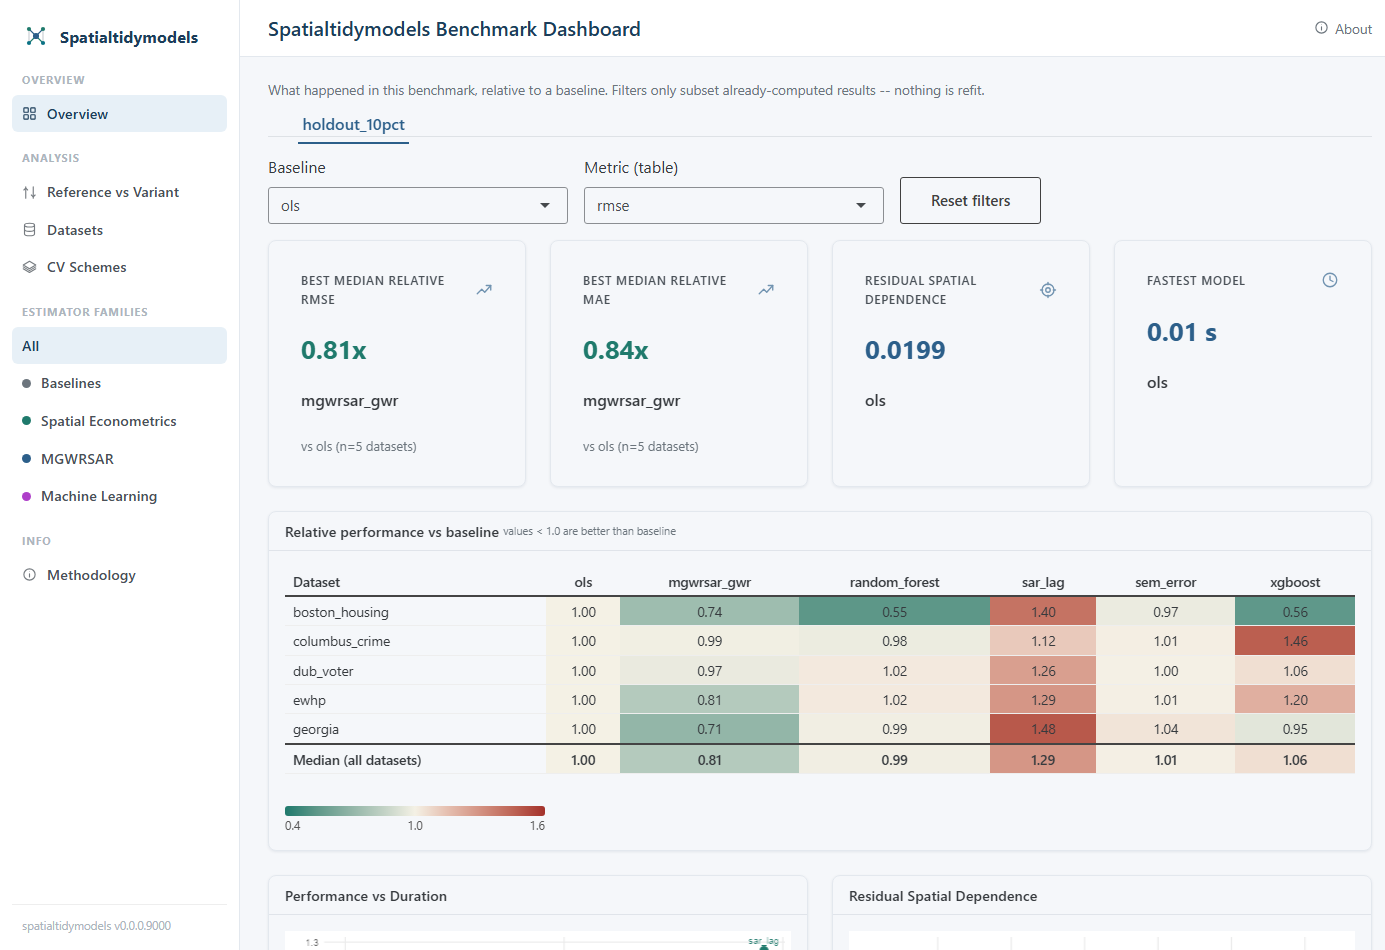
\includegraphics[width=0.90\textwidth]{dashboard_screenshot.png}
    \caption{Tableau de bord interactif de \texttt{spatialtidymodels}.}
    \label{fig:dashboard}
\end{figure}

\subsection{Difficultés rencontrées et démarche de diagnostic}

Les difficultés rencontrées au cours de la mission ne constituent pas une liste exhaustive des problèmes possibles. Elles illustrent plutôt la démarche adoptée pour faire évoluer le projet. Lorsqu'un cas particulier était identifié, l'objectif n'était pas seulement de le corriger manuellement, mais d'en comprendre l'origine, d'isoler l'étape concernée et, lorsque cela était possible, de modifier les règles du pipeline afin de réduire les interventions humaines lors des exécutions suivantes.

La première version du dispositif est volontairement focalisée sur les données spatiales en coupe transversale, avec une variable réponse continue. Des jeux de données de panel ont été recensés et documentés, mais ils ne sont pas intégrés au benchmark principal. Leur traitement suppose des règles spécifiques pour prendre en compte simultanément les unités spatiales et la dimension temporelle. Ce choix de périmètre permet de stabiliser l'infrastructure sur un premier cas d'usage avant d'envisager son extension.

L'automatisation de la préparation des fiches peut produire des erreurs qui n'interrompent pas l'exécution des scripts. Une fiche peut être techniquement complète tout en contenant une information incorrecte sur une variable, une formule ou le type de jeu de données. La vérification de certaines fiches par confrontation avec les données et l'article source m'a ainsi permis d'identifier, dans un jeu épidémiologique, une p-valeur du test de Mann-Kendall enregistrée comme covariable en plus de la statistique dont elle était issue. Ce type de cas a montré que la présence des champs attendus ne suffit pas à garantir la validité des métadonnées. Les contrôles automatiques peuvent signaler des incohérences, mais les cas ambigus doivent encore faire l'objet d'une vérification ciblée.

La récupération des sources a constitué une autre limite pratique. L'assistant IA peut utiliser les scripts et les outils du projet pour explorer et organiser le corpus, mais certains sites bloquent les téléchargements automatisés. Des jeux de données ou des PDF ont alors dû être récupérés manuellement lorsqu'ils étaient librement accessibles. D'autres candidats intéressants n'ont pas été retenus lorsque l'article ou les données étaient payants, ou lorsqu'ils exigeaient la création d'un compte. Ce choix est cohérent avec l'objectif de constituer une ressource dont les données, les sources et les procédures de reproduction restent accessibles librement.

La détection systématique des doublons à tous les niveaux a également constitué un point de vigilance. Un même jeu de données peut apparaître dans plusieurs packages, sous des noms différents ou dans des versions proches. Les scripts combinent donc des contrôles sur le nom, la structure des données et leur provenance. Ils détectent automatiquement les doublons manifestes et signalent les rapprochements incertains pour examen. Cette prudence est nécessaire, car une règle trop stricte risquerait de fusionner des jeux distincts partageant seulement certaines caractéristiques.

Enfin, les tests de validation croisée ont révélé des difficultés invisibles lors d'un ajustement sur les seules données d'apprentissage. Un estimateur pouvait être ajusté correctement, mais échouer à produire des prédictions exploitables sur un ensemble de test. Cette observation a conduit à séparer plus nettement les étapes d'ajustement, de prédiction et de calcul des métriques.

Ces exemples montrent que la robustesse du dispositif repose autant sur les règles de préparation et les contrôles du pipeline que sur l'exécution des scripts eux-mêmes. L'automatisation ne supprime pas toute vérification humaine, mais elle permet de réserver celle-ci aux cas réellement ambigus et de conserver une trace des décisions prises.


\subsection{État actuel, contribution et utilité du dispositif}

Le projet a produit deux composantes complémentaires : un catalogue documenté de jeux de données et une infrastructure permettant de les exploiter dans des benchmarks. Le tableau~\ref{tab:composition-catalogue} présente la composition actuelle du catalogue et les principaux états de préparation des jeux.

\begin{table}[h]
\centering
\small
\begin{tabular}{lrr}
\toprule
& Effectif & Part \\
\midrule
\multicolumn{3}{l}{\textit{Par voie initiale d'intégration}} \\
Jeux issus d'entrepôts scientifiques & 153 & 53\,\% \\
Jeux distribués par des packages R & 76 & 26\,\% \\
Jeux distribués par des packages Python & 62 & 21\,\% \\
\midrule
\multicolumn{3}{l}{\textit{Par statut de sélection}} \\
Retenus pour intégration au package & 155 & 53\,\% \\
En révision manuelle & 55 & 19\,\% \\
Écartés du périmètre & 81 & 28\,\% \\
\midrule
\multicolumn{3}{l}{\textit{Par état opérationnel}} \\
Benchmark-ready & 117 & 40\,\% \\
Exemples embarqués dans le package & 16 & 5\,\% \\
\midrule
\multicolumn{3}{l}{\textit{Par structure spatiale}} \\
Coupe transversale (spatial pur) & 239 & 82\,\% \\
Panel spatio-temporel & 52 & 18\,\% \\
\midrule
\multicolumn{3}{l}{\textit{Licence, parmi les jeux retenus}} \\
Licence identifiée et tracée à la source & 152 & 98\,\% \\
Licence non identifiée ou non renseignée & 3 & 2\,\% \\
\bottomrule
\end{tabular}
\caption{Composition du catalogue de jeux de données.}
\label{tab:composition-catalogue}
\end{table}

Ces catégories correspondent à des étapes distinctes du parcours des jeux dans le projet. L'intégration au package et le statut \texttt{benchmark\_ready} ne constituent pas, à eux seuls, des résultats de benchmark.

\clearpage
Le tableau~\ref{tab:jeux-diversite} illustre la diversité des jeux retenus. Les exemples couvrent plusieurs domaines et disposent d'une spécification empirique reliée à une publication scientifique.

\begin{table}[H]
\centering
\footnotesize
\begin{tabularx}{\textwidth}{@{}p{2.6cm}p{2.0cm}rXrp{2.6cm}p{1.8cm}@{}}
\toprule
Jeu de données & Domaine & N & Réponse Y & X & Source (DOI) & Nb. estim. éligibles \\
\midrule
Boston housing & Immobilier & 506 & valeur médiane du logement, continue & 13 & \url{https://doi.org/10.1016/0095-0696(78)90006-2} & \BostonEligibleCount \\
Diabète et confusion spatiale & Santé publique & 2\,984 & prévalence du diabète, continue & 16 & \url{https://doi.org/10.5281/zenodo.21300380} & \DiabetesEligibleCount \\
Dragonfly diversity Europe & Macroécologie & 4\,192 & richesse spécifique, comptage & 3 & \url{https://doi.org/10.5061/dryad.78j8g} & \DragonflyEligibleCount \\
Florida crash GSVCM & Transport & 11\,249 & nombre d'accidents, comptage & 6 & \url{https://doi.org/10.6084/m9.figshare.12156975} & \FloridaEligibleCount \\
Seshat social complexity & Histoire quantitative & 307 & population de la polity, continue & 3 & \url{https://doi.org/10.17916/p6159w} & \SeshatEligibleCount \\
Airbnb Europe prices & Économie urbaine & 51\,707 & prix logarithmé, continue & 12 & \url{https://doi.org/10.5281/zenodo.4446043} & \AirbnbEligibleCount \\
\bottomrule
\end{tabularx}
\vspace{0.15cm}

\raggedright\scriptsize Note : la colonne indique le nombre de routes que les métadonnées autorisent à tester ; elle ne constitue pas encore un résultat de performance.
\caption{Exemples de jeux de données issus de domaines différents.}
\label{tab:jeux-diversite}
\end{table}

Le développement de \texttt{spatialtidymodels} a permis de relier ce catalogue à une infrastructure commune d'estimation, de validation et de comparaison. Les tests réalisés au cours du développement ont également permis d'identifier plusieurs erreurs dans l'orchestration des benchmarks, notamment sur la prédiction hors échantillon, la récupération des paramètres spatiaux et le calcul des métriques après concaténation des prédictions.

Ma contribution a principalement porté sur la structuration du système de métadonnées, le développement et l'amélioration des pipelines de collecte et de curation, l'organisation du corpus autour du wiki et du graphe de connaissances, ainsi que le développement de \texttt{spatialtidymodels} et de ses outils de benchmark.


La banque permet à un chercheur qui développe une nouvelle méthode de l'évaluer sur un large éventail de jeux de données empiriques. En complément des simulations de Monte Carlo, il peut sélectionner des jeux adaptés à sa méthode et observer son comportement dans plusieurs contextes empiriques. Cette démarche permet de produire, dans un article méthodologique, une validation plus robuste qu'une évaluation fondée sur un nombre très limité d'applications.

Le package \texttt{spatialtidymodels} complète cet usage en fournissant un cadre commun de comparaison. Il permet de confronter l'estimateur proposé à des méthodes de référence dans les mêmes conditions. Les jeux préparés, les règles d'éligibilité, les schémas de séparation et les métriques sont partagés.

Pour le labo, le dispositif rassemble un travail coûteux de recherche, de préparation et de documentation des données. Lorsqu'une nouvelle méthode est développée, il devient possible de s'appuyer sur une ressource déjà structurée plutôt que de recommencer ces étapes. La banque et le package pourront ainsi servir de support commun aux travaux méthodologiques de l'unité et à leur diffusion ouverte.

% ============================ CONCLUSION ET PERSPECTIVES ============================
\section{Conclusion et perspectives}

Lorsqu'une nouvelle méthode spatiale est proposée, il faut pouvoir vérifier qu'elle fonctionne au-delà des exemples pour lesquels elle a été conçue. Les simulations de Monte Carlo sont utiles, car elles permettent de tester une méthode dans des situations contrôlées. Toutefois, elles ne suffisent pas à représenter toute la diversité des problèmes rencontrés dans des données réelles. Dans les articles, les applications reposent souvent sur seulement deux ou trois jeux empiriques, choisis et préparés pour l'étude. Il devient alors difficile de savoir si les résultats restent vrais dans d'autres contextes, ou de comparer plusieurs méthodes de manière équitable. C'est ce manque de jeux de données réelles, variées et documentées qui a motivé la mission.

Pour répondre à ce besoin, nous avons réuni plusieurs outils complémentaires : des scripts R, un wiki, un graphe de connaissances, des règles de contrôle et une infrastructure de benchmark. Des LLM ont également été utilisés de manière encadrée pour soutenir ce travail. Chaque jeu est associé à des métadonnées utiles à sa réutilisation, notamment sa source, sa variable réponse, ses covariables, une formule de régression identifiée dans un papier scientifique lorsqu'elle est disponible, sa structure spatiale, sa licence et les estimateurs qui peuvent lui être appliqués. Ces informations permettent de sélectionner les jeux appropriés et de guider l'évaluation des méthodes de manière unifiée.

La suite immédiate du projet consiste à relancer les pipelines de collecte et de traitement par lots. Les jeux candidats seront recherchés, récupérés lorsqu'ils sont librement accessibles, documentés, contrôlés puis promus dans le registre du package lorsque les informations nécessaires sont disponibles. L'idée est d'élargir progressivement la banque jusqu'à couvrir un ensemble assez exhaustif de configurations.

À terme, le package conservera les codes, le registre des estimateurs, les procédures de benchmark et un nombre limité de jeux d'exemple nécessaires à son fonctionnement autonome. Pour éviter d'alourdir son installation, la banque complète sera déposée séparément dans un dépôt ouvert, versionné et citable. Les utilisateurs pourront télécharger, depuis le package, les jeux supplémentaires dont ils ont besoin pour exécuter un benchmark. Le choix définitif de l'entrepôt devra tenir compte des licences, des conditions de redistribution et des possibilités d'hébergement du laboratoire.

La banque de données finalisée fera l'objet d'une publication scientifique sous la forme d'un \textit{data paper} de type \textit{Data Descriptor} dans \textit{Scientific Data}, qui décrira la ressource, sa construction et ses conditions de réutilisation, sans présenter de classement des estimateurs.

Le \textit{data paper} inclura également une étude bibliométrique sur la place des données réelles dans les articles qui proposent de nouvelles méthodes spatiales. Son objectif sera de comparer l'effort consacré aux configurations de Monte-Carlo avec le nombre de jeux empiriques réellement utilisés pour évaluer les méthodes. Le corpus actuel servira de pilote ; une base d'articles méthodologiques plus large et stratifiée devra ensuite être constituée pour produire des résultats publiables.

L'extension de la banque permettra enfin d'intégrer de nouvelles familles d'estimateurs lorsque des jeux adaptés et des routes d'évaluation stabilisées seront disponibles. Les réponses binaires, les comptages et les données de panel constituent des prolongements naturels. Les modèles spatiaux binaires, notamment de type probit, ainsi que les modèles adaptés aux comptages, pourront alors être ajoutés sans confondre ces développements futurs avec les capacités actuellement disponibles.

Le cursus de Master a constitué un appui direct pour ce travail, en particulier par les enseignements d'économétrie, de programmation et d'intelligence artificielle. Le stage m'a permis de développer une pratique plus intégrée de la recherche reproductible, associant traitement de données, développement R, contrôle des sources et usage encadré d'assistants IA. Il a également renforcé l'importance du diagnostic et de la vérification : l'automatisation facilite le traitement d'un corpus volumineux, mais elle ne remplace ni la validation des informations ni le jugement méthodologique.

% ============================ ANNEXES ============================
\clearpage
\appendix

\section{Annexe 1 : Synthèse technique du pipeline}
\label{annexe:pipeline}

Cette annexe résume les éléments techniques qui sous-tendent le rapport. Elle ne remplace pas la documentation du dépôt, mais donne une vue d'ensemble du chemin suivi par un jeu candidat avant son utilisation dans \texttt{spatialtidymodels}.

\subsection{Trois pipelines de collecte}

Le projet combine trois voies de collecte. Elles ne produisent pas directement les mêmes objets, mais convergent vers les mêmes couches de curation : fiches wiki, objets spatiaux \texttt{sf}, graphe de connaissances et registre du package.

\begin{figure}[H]
\centering
\resizebox{\textwidth}{!}{%
\begin{tikzpicture}[
  node distance=0.75cm and 0.8cm,
  every node/.style={font=\scriptsize, align=center},
  source/.style={draw=myblue!70, fill=blue!6, rounded corners, text width=4.2cm, minimum height=1.05cm},
  pipeStep/.style={draw=mygray!70, fill=black!3, rounded corners, text width=4.2cm, minimum height=1.05cm},
  output/.style={draw=mygreen!75, fill=mygreen!8, rounded corners, text width=4.2cm, minimum height=1.05cm},
  final/.style={draw=myred!75, fill=myred!8, rounded corners, text width=5.4cm, minimum height=1.05cm},
  arr/.style={-{Latex[length=2mm]}, thick, mygray}
]
\node[source] (src) {Sources de jeux de données};

\node[source, below left=1.0cm and 5.2cm of src] (datacite) {Pipeline DataCite\\métadonnées de dépôts indexés};
\node[source, below=1.0cm of src] (papers) {Pipeline articles scientifiques\\DataCite, revues, Dryad ou Zenodo};
\node[source, below right=1.0cm and 5.2cm of src] (packages) {Pipeline packages\\R et Python};

\node[pipeStep, below=0.65cm of datacite] (datacite2) {Filtrage, dédoublonnage, enrichissement\\Crossref et OpenAlex};
\node[pipeStep, below=0.65cm of papers] (papers2) {PDF, données brutes, BibTeX\\et conversion GROBID};
\node[pipeStep, below=0.65cm of packages] (packages2) {Extraction et inspection locale\\des objets distribués};

\node[pipeStep, below=0.65cm of papers2] (kg) {Curation et preuves\\dans le graphe de connaissances};
\node[pipeStep, below=0.65cm of packages2] (pkgdoc) {Documentation et audit\\des sources};

\node[output, below=1.25cm of kg, xshift=-2.5cm] (wiki) {Fiches wiki de jeux\\et contrôle qualité};
\node[output, below=1.25cm of kg, xshift=2.5cm] (sf) {Objets spatiaux \texttt{sf}\\et métadonnées normalisées};

\node[final, below=0.85cm of kg, yshift=-3.0cm] (registry) {Registre \texttt{spatialtidymodels}\\\texttt{package\_include}: \texttt{yes}, \texttt{manual\_review}, \texttt{no}};
\node[final, below=0.7cm of registry] (bench) {Benchmark reproductible\\des estimateurs spatiaux};

\draw[arr] (src) -- (datacite);
\draw[arr] (src) -- (papers);
\draw[arr] (src) -- (packages);
\draw[arr] (datacite) -- (datacite2);
\draw[arr] (papers) -- (papers2);
\draw[arr] (packages) -- (packages2);
\draw[arr] (datacite2) |- (kg);
\draw[arr] (papers2) -- (kg);
\draw[arr] (packages2) -- (pkgdoc);
\draw[arr] (pkgdoc) |- (kg);
\draw[arr] (kg) -- (wiki);
\draw[arr] (kg) -- (sf);
\draw[arr] (wiki) -- (registry);
\draw[arr] (sf) -- (registry);
\draw[arr] (registry) -- (bench);
\end{tikzpicture}}
\caption{Convergence des trois pipelines de collecte vers le registre de benchmark.}
\end{figure}

Le pipeline DataCite est un mécanisme de découverte et de préqualification : il exploite les métadonnées des dépôts, filtre les candidats et les enrichit, mais ne rend pas automatiquement un jeu utilisable. Le pipeline des articles scientifiques reprend ces candidats, ou ceux issus d'une recherche par revue, puis vérifie les preuves dans le PDF et les données. Le pipeline packages part d'objets déjà distribués dans des bibliothèques R ou Python et les documente à partir de leur inspection locale et de leurs sources.

\subsection{Chemin d'un jeu de données issu d'un papier}

\begin{center}
\small
\begin{tabularx}{\textwidth}{>{\bfseries}p{3.2cm}X}
\toprule
Étape & Rôle dans le projet \\
\midrule
Collecte & Recherche de candidats via DataCite, Dryad, Zenodo ou revues spécialisées. \\
Récupération & Téléchargement légal du PDF et des fichiers de données lorsque ceux-ci sont disponibles. \\
Bibliographie & Création ou correction de l'entrée BibTeX, avec DOI, auteurs, titre et lien vers le PDF local. \\
GROBID & Conversion du PDF en TEI pour accéder aux sections, tableaux, références et mentions de données. \\
KG & Création des relations entre papier, jeu de données, formule, variables, source et statut de curation. \\
Loader R & Transformation des fichiers bruts en objet \texttt{sf} reproductible. \\
Fiche Markdown & Documentation homogène du jeu, de sa provenance, des variables et des estimateurs éligibles. \\
Vérification & Contrôle croisé entre papier, TEI, données locales et fiche ; aucune formule n'est promue sans preuve. \\
Package & Export vers les métadonnées de \texttt{spatialtidymodels} si le statut \texttt{benchmark\_ready} est atteint. \\
\bottomrule
\end{tabularx}
\end{center}

\subsection{Rôle du graphe de connaissances}

Le graphe de connaissances sert de couche intermédiaire entre les sources brutes et les fiches finales. Il ne remplace pas le papier ou les données, mais conserve les relations utiles au raisonnement : quel papier mentionne quel jeu, quelle formule est associée à quelle réponse, quelles covariables sont documentées, quelle source a permis de récupérer les fichiers et quel statut de préparation a été attribué. Cette organisation évite de relire entièrement le corpus à chaque étape et rend les décisions de curation plus traçables.

\begin{figure}[H]
\centering
\resizebox{0.97\textwidth}{!}{%
\begin{tikzpicture}[
  node distance=0.8cm and 1.0cm,
  every node/.style={font=\scriptsize, align=center},
  dataset/.style={draw=mygreen!80, fill=mygreen!10, rounded corners, minimum width=3.2cm, minimum height=0.85cm, font=\scriptsize\bfseries},
  paper/.style={draw=myblue!70, fill=blue!7, rounded corners, text width=3.0cm, minimum height=0.9cm},
  package/.style={draw=violet!70, fill=violet!7, rounded corners, text width=2.9cm, minimum height=0.85cm},
  formula/.style={draw=myred!75, fill=myred!7, rounded corners, text width=4.8cm, minimum height=0.85cm},
  varnode/.style={draw=mygray!65, fill=black!3, rounded corners, text width=2.7cm, minimum height=0.75cm},
  decision/.style={draw=orange!80!black, fill=orange!9, rounded corners, text width=3.5cm, minimum height=0.85cm},
  edge/.style={-{Latex[length=1.8mm]}, thick, mygray}
]
\node[dataset] (lsl) {\texttt{spDataLarge::lsl}};
\node[package, left=2.0cm of lsl] (pkg) {package R\\\texttt{spDataLarge}};
\node[paper, above left=1.0cm and 0.7cm of lsl] (article) {Muenchow, Brenning\\et Richter (2012)};
\node[paper, above right=1.0cm and 0.7cm of lsl] (book) {\emph{Geocomputation with R}\\chapitre spatial-cv};
\node[varnode, right=2.0cm of lsl] (sf) {objet \texttt{sf}\\350 points\\EPSG:32717};
\node[formula, below=1.0cm of lsl] (form) {\texttt{lslpts} $\sim$ \texttt{slope + cplan + cprof}\\\texttt{+ elev + log10\_carea}};
\node[varnode, below left=0.8cm and 1.0cm of form] (y) {\texttt{lslpts}\\réponse binaire};
\node[varnode, below=0.8cm of form] (x) {\texttt{slope}, \texttt{cplan}, \texttt{cprof},\\\texttt{elev}, \texttt{log10\_carea}};
\node[varnode, below right=0.8cm and 1.0cm of form] (coord) {\texttt{x}, \texttt{y}\\coordonnées exclues de X};
\node[decision, below=1.1cm of x] (ready) {\texttt{package\_include: no}\\réponse non continue\\pour le benchmark actuel};

\draw[edge] (pkg) -- node[above]{fournit} (lsl);
\draw[edge] (article) -- node[left]{documente} (lsl);
\draw[edge] (book) -- node[right]{réutilise} (lsl);
\draw[edge] (lsl) -- node[above]{matérialisé par} (sf);
\draw[edge,myred] (lsl) -- node[right]{formule retenue} (form);
\draw[edge] (form) -- (y);
\draw[edge] (form) -- (x);
\draw[edge] (form) -- (coord);
\draw[edge] (y) -- (ready);
\draw[edge] (x) -- (ready);
\end{tikzpicture}}
\caption{Sous-graphe simplifié centré sur le jeu \texttt{spDataLarge::lsl}.}
\label{fig:kg-lsl}
\end{figure}

L'exemple LSL montre pourquoi le graphe ne sert pas seulement à accumuler des liens. Le jeu est bien documenté : il provient de \texttt{spDataLarge}, contient 350 observations ponctuelles dans le sud de l'Équateur, cinq covariables topographiques et une formule reliée à la publication de Muenchow, Brenning et Richter (2012). En revanche, la variable \texttt{lslpts} indique une présence ou absence de glissement de terrain. Le KG conserve donc simultanément la preuve d'existence du jeu, la formule exploitable et la raison de non-promotion dans le benchmark de régression continue actuel.

\subsection{Structure attendue d'une fiche de jeu}

Une fiche utilisable pour le benchmark doit contenir au minimum : la provenance du jeu, le DOI du papier ou de la source lorsqu'il existe, la variable réponse, les covariables retenues, la formule publiée ou reconstruite, le support spatial, les informations de licence, le statut de préparation et le bloc d'éligibilité des estimateurs. Les champs manquants ne doivent pas être complétés par hypothèse ; ils restent documentés comme limites ou motifs de révision.

\subsection{Exemple de fiche complète}

Le jeu \texttt{paper\_airbnb\_europe\_prices} illustre le niveau attendu pour promouvoir un jeu vers le registre du package. Il provient de l'article de Gyodi et Nawaro (2021) sur les déterminants spatiaux des prix Airbnb en Europe et des fichiers déposés sur Zenodo. La fiche associe la source bibliographique, le dépôt de données, la formule empirique, les variables disponibles localement et les estimateurs éligibles.

\begin{center}
\small
\begin{tabularx}{\textwidth}{>{\bfseries}p{3.8cm}X}
\toprule
Élément contrôlé & Contenu retenu dans la fiche \\
\midrule
Source & Article \emph{Determinants of Airbnb prices in European cities: A spatial econometrics approach}, DOI \texttt{10.1016/j.tourman.2021.104319}. \\
Données & Dépôt Zenodo \texttt{10.5281/zenodo.4446043}, 51\,707 annonces Airbnb, 10 villes européennes, coordonnées \texttt{lng}/\texttt{lat}. \\
Réponse & \texttt{log\_price}, logarithme du prix, variable continue utilisée dans le papier. \\
Covariables & Type de logement, capacité, statut de l'hôte, professionnalisation, notes, chambres, distance au centre, distance au métro, attractivité touristique et restaurants. \\
Formule système & \texttt{log\_price} $\sim$ \texttt{room\_type + person\_capacity + host\_is\_superhost + multi + biz + cleanliness\_rating + guest\_satisfaction\_overall + bedrooms + dist + metro\_dist + attr\_index + rest\_index}. \\
Support spatial & Points en WGS84, matrice de voisinage reconstruite par le benchmark selon le schéma d'évaluation. \\
Statut & \texttt{benchmark\_status: ready}, \texttt{package\_include: yes}. \\
Estimateurs éligibles & Références globales, modèles SAR/SEM/SDM, GWR et méthodes prédictives non linéaires documentées comme routes de benchmark. \\
\bottomrule
\end{tabularx}
\end{center}

Cet exemple montre la différence entre une fiche simplement descriptive et une fiche utilisable : les champs ne se limitent pas à l'existence d'un fichier spatial, mais relient explicitement le jeu, l'article, la formule, les variables réellement présentes et la décision d'éligibilité.

\subsection{Estimateurs actuellement recensés}

Le registre du package contient 28 estimateurs ou variantes, regroupés de la manière suivante.

\begin{center}
\scriptsize
\begin{tabularx}{\textwidth}{>{\bfseries}p{3.2cm}X}
\toprule
Famille & Estimateurs ou variantes \\
\midrule
Références globales & \texttt{ols}, \texttt{earth}, \texttt{earth\_xy}, \texttt{gam\_spatial} \\
SAR, SEM, SDM & \texttt{sar\_lag}, \texttt{sem\_error}, \texttt{sdm\_mixed} \\
GWR et MGWRSAR & \texttt{mgwrsar\_gwr}, \texttt{mgwrsar\_mgwr}, \texttt{mgwrsar\_sar}, \texttt{mgwrsar\_mgwrsar}, \texttt{MGWRSAR\_0\_kc\_kv}, \texttt{MGWRSAR\_1\_kc\_kv} \\
Boosting & \texttt{gamboost}, \texttt{spboost}, \texttt{spboost\_bspa\_sar\_ml}, \texttt{spboost\_bspa\_sar\_cfe}, \texttt{spboost\_bspa\_sem\_ml}, \texttt{spboost\_bspa\_sem\_cfe} \\
Forêts et gradient boosting & \texttt{random\_forest}, \texttt{random\_forest\_xy}, \texttt{xgboost}, \texttt{xgboost\_xy}, \texttt{spatialml\_grf}, \texttt{spatialrf}, \texttt{rfgls} \\
Filtres spatiaux & \texttt{spmoran\_esf}, \texttt{spmoran\_resf} \\
\bottomrule
\end{tabularx}
\end{center}

Tous ne répondent pas à la même logique statistique. Certains estiment un paramètre spatial explicite, d'autres exploitent l'information géographique par les covariables, et d'autres servent de références non spatiales. Cette distinction est conservée dans les résultats du benchmark.

\begin{center}
\scriptsize
\begin{tabularx}{\textwidth}{>{\bfseries}p{2.7cm}p{4.0cm}X}
\toprule
Famille conceptuelle & Écriture schématique & Rôle dans le benchmark \\
\midrule
Régression globale & $y = X\beta + \varepsilon$ & Référence non spatiale, utile pour mesurer le gain éventuel des modèles spatiaux. \\
SAR lag & $y = \rho Wy + X\beta + \varepsilon$ & Modélise une dépendance directe de la réponse entre unités voisines. \\
SEM error & $y = X\beta + u,\quad u=\lambda Wu+\varepsilon$ & Modélise l'autocorrélation dans le terme d'erreur. \\
SDM & $y = \rho Wy + X\beta + WX\theta + \varepsilon$ & Combine dépendance sur la réponse et effets des covariables voisines. \\
GWR / MGWR & $y_i = X_i\beta(s_i)+\varepsilon_i$ & Autorise des coefficients variables dans l'espace ; MGWR permet plusieurs échelles spatiales. \\
Forêts, boosting et MARS & $y = f(X,\mathrm{coords})+\varepsilon$ & Références prédictives non linéaires ; l'information spatiale peut entrer par coordonnées ou variables dérivées. \\
Filtres spatiaux & $y = X\beta + E\gamma + \varepsilon$ & Ajoutent des composantes spatiales, par exemple des vecteurs propres de Moran. \\
\bottomrule
\end{tabularx}
\end{center}

La taxonomie doit encore être stabilisée dans les métadonnées du package. La convention utile est de distinguer trois niveaux : la famille statistique générique, le moteur logiciel utilisé et la route concrète du benchmark. Par exemple, un estimateur peut appartenir à la famille SAR, être ajusté par le package \texttt{spboost}, et apparaître dans le tableau de bord sous une route explicite comme \texttt{spboost\_bspa\_sar\_ml}. Cette séparation évite de mélanger méthode, package et variante d'implémentation.

\subsection{Outils utiles aux assistants IA}

Le dépôt contient aussi des outils destinés à rendre le travail des assistants plus contrôlable. Les serveurs MCP locaux donnent accès à des fonctions spécialisées sans relire tout le dépôt : recherche dans le catalogue de jeux, mémoire de code, compression de sorties terminal, gestion du contexte et requêtes compactes. Les compétences de Matt Pocock installées localement servent plutôt à structurer le travail d'ingénierie : revue de code, diagnostic de bogues, modélisation de domaine, conception de modules, rédaction pédagogique, développement piloté par les tests et transformation d'un plan en tâches.

\begin{center}
\small
\begin{tabularx}{\textwidth}{>{\bfseries}p{3.5cm}X}
\toprule
Famille d'outils & Usage dans le projet \\
\midrule
MCP \texttt{dataset\_search} & Interroger rapidement le catalogue de jeux et éviter de relire les fiches une par une. \\
MCP \texttt{codebase\_memory} & Repérer les fichiers, fonctions, imports et dépendances utiles dans le code. \\
MCP \texttt{context\_store}, \texttt{rtk}, \texttt{headroom} & Résumer de longues sorties terminal ou de grands blocs de contexte avant raisonnement. \\
Compétences de revue et diagnostic & \texttt{code-review}, \texttt{diagnosing-bugs}, \texttt{tdd} pour contrôler les modifications et stabiliser les scripts. \\
Compétences de conception & \texttt{domain-modeling}, \texttt{codebase-design}, \texttt{teach}, \texttt{to-prd}, \texttt{to-issues} pour formaliser le vocabulaire, les décisions et les tâches. \\
\bottomrule
\end{tabularx}
\end{center}


\clearpage


% ============================ REFERENCES ============================
\section*{Références}

{\small
\RaggedRight
\setlength{\parindent}{0pt}
\setlength{\parskip}{0.12cm}

\textbf{Méthodes spatiales et spatio-temporelles}\\[0.15cm]

Anselin, L. (1988). \textit{Spatial Econometrics: Methods and Models}. Dordrecht: Springer. \url{https://doi.org/10.1007/978-94-015-7799-1}\\[0.2cm]

Bivand, R., Millo, G. \& Piras, G. (2021). A review of software for spatial econometrics in R. \textit{Mathematics}, 9(11), 1276. \url{https://doi.org/10.3390/math9111276}\\[0.2cm]

Brunsdon, C., Fotheringham, A. S. \& Charlton, M. E. (1996). Geographically weighted regression: a method for exploring spatial nonstationarity. \textit{Geographical Analysis}, 28(4), 281--298. \url{https://doi.org/10.1111/j.1538-4632.1996.tb00936.x}\\[0.2cm]

Casetti, E. (1972). Generating models by the expansion method: applications to geographical research. \textit{Geographical Analysis}, 4(1), 81--91. \url{https://doi.org/10.1111/j.1538-4632.1972.tb00458.x}\\[0.2cm]

Cliff, A. D. \& Ord, J. K. (1973). \textit{Spatial Autocorrelation}. London: Pion.\\[0.2cm]

Fotheringham, A. S., Yang, W. \& Kang, W. (2017). Multiscale geographically weighted regression (MGWR). \textit{Annals of the American Association of Geographers}, 107(6), 1247--1265. \url{https://doi.org/10.1080/24694452.2017.1352480}\\[0.2cm]

Geniaux, G. \& Martinetti, D. (2018). A new method for dealing simultaneously with spatial autocorrelation and spatial heterogeneity in regression models. \textit{Regional Science and Urban Economics}, 72, 74--85. \url{https://doi.org/10.1016/j.regsciurbeco.2017.04.001}\\[0.2cm]

Geniaux, G. (2023). Functional gradient descent boosting for additive non-linear spatial autoregressive model (gaussian and probit). \textit{HAL}, hal-04229868. \url{https://hal.inrae.fr/hal-04229868}\\[0.2cm]

Geniaux, G. (2026a). \textit{spboost: Gradient Boosting for Nonlinear Spatial Autoregressive Models}. R package version 0.7.0. \url{https://doi.org/10.32614/CRAN.package.spboost}\\[0.2cm]

Geniaux, G. (2026). Top-down scale approaches for multiscale GWR with locally adaptive bandwidths. \textit{Journal of Geographical Systems}, 28, 27--76. \url{https://doi.org/10.1007/s10109-025-00481-4}\\[0.2cm]

Lee, L.-F. (2004). Asymptotic distributions of quasi-maximum likelihood estimators for spatial autoregressive models. \textit{Econometrica}, 72(6), 1899--1925. \url{https://doi.org/10.1111/j.1468-0262.2004.00558.x}\\[0.2cm]

Le Gallo, J. (2002). Économétrie spatiale 1. Autocorrélation spatiale. \textit{Économie \& Prévision}, 155(4), 139--157. \url{https://doi.org/10.3406/ecop.2002.6875}\\[0.2cm]

Le Gallo, J. (2004). Économétrie spatiale 2. Hétérogénéité spatiale. \textit{Économie \& Prévision}, 162(1), 151--174. \url{https://doi.org/10.3917/ecop.162.0151}\\[0.2cm]

Legendre, P. (1993). Spatial autocorrelation: trouble or new paradigm? \textit{Ecology}, 74(6), 1659--1673. \url{https://doi.org/10.2307/1939924}\\[0.2cm]

Lindgren, F., Rue, H. \& Lindström, J. (2011). An explicit link between Gaussian fields and Gaussian Markov random fields: the stochastic partial differential equation approach. \textit{Journal of the Royal Statistical Society: Series B}, 73(4), 423--498. \url{https://doi.org/10.1111/j.1467-9868.2011.00777.x}\\[0.2cm]

Murakami, D. \& Griffith, D. A. (2019). Eigenvector spatial filtering for large data sets: fixed and random effects approaches. \textit{Geographical Analysis}, 51(1), 23--49. \url{https://doi.org/10.1111/gean.12156}\\[0.4cm]

Martinetti, D. \& Geniaux, G. (2017). Approximate likelihood estimation of spatial probit models. \textit{Regional Science and Urban Economics}, 64, 30--45. \url{https://doi.org/10.1016/j.regsciurbeco.2017.02.002}\\[0.4cm]

\textbf{Estimateurs statistiques et apprentissage automatique}\\[0.15cm]

Breiman, L. (2001). Random forests. \textit{Machine Learning}, 45, 5--32. \url{https://doi.org/10.1023/A:1010933404324}\\[0.2cm]

Bühlmann, P. \& Hothorn, T. (2007). Boosting algorithms: regularization, prediction and model fitting. \textit{Statistical Science}, 22(4), 477--505. \url{https://doi.org/10.1214/07-STS242}\\[0.2cm]

Chen, T. \& Guestrin, C. (2016). XGBoost: a scalable tree boosting system. In \textit{Proceedings of the 22nd ACM SIGKDD International Conference on Knowledge Discovery and Data Mining}, 785--794. \url{https://doi.org/10.1145/2939672.2939785}\\[0.2cm]

Friedman, J. H. (1991). Multivariate adaptive regression splines. \textit{The Annals of Statistics}, 19(1), 1--67. \url{https://doi.org/10.1214/aos/1176347963}\\[0.2cm]

Wood, S. N. (2003). Thin plate regression splines. \textit{Journal of the Royal Statistical Society: Series B}, 65(1), 95--114. \url{https://doi.org/10.1111/1467-9868.00374}\\[0.2cm]

Nelder, J. A. \& Wedderburn, R. W. M. (1972). Generalized linear models. \textit{Journal of the Royal Statistical Society: Series A}, 135(3), 370--384. \url{https://doi.org/10.2307/2344614}\\[0.4cm]

\textbf{Évaluation, comparaison de méthodes et validation croisée spatiale}\\[0.15cm]

Demšar, J. (2006). Statistical comparisons of classifiers over multiple data sets. \textit{Journal of Machine Learning Research}, 7, 1--30. \url{https://www.jmlr.org/papers/v7/demsar06a.html}\\[0.2cm]

Olson, R. S., La Cava, W., Orzechowski, P., Urbanowicz, R. J. \& Moore, J. H. (2017). PMLB: a large benchmark suite for machine learning evaluation and comparison. \textit{BioData Mining}, 10, 36. \url{https://doi.org/10.1186/s13040-017-0154-4}\\[0.2cm]

Roberts, D. R., Bahn, V., Ciuti, S., Boyce, M. S., Elith, J., Guillera-Arroita, G. \textit{et al.} (2017). Cross-validation strategies for data with temporal, spatial, hierarchical, or phylogenetic structure. \textit{Ecography}, 40(8), 913--929. \url{https://doi.org/10.1111/ecog.02881}\\[0.2cm]

Schratz, P., Muenchow, J., Iturritxa, E., Richter, J. \& Brenning, A. (2019). Hyperparameter tuning and performance assessment of statistical and machine-learning algorithms using spatial data. \textit{Ecological Modelling}, 406, 109--120. \url{https://doi.org/10.1016/j.ecolmodel.2019.06.002}\\[0.2cm]

Thiyagalingam, J., Shankar, M., Fox, G. \& Hey, T. (2022). Scientific machine learning benchmarks. \textit{Nature Reviews Physics}, 4, 413--420. \url{https://doi.org/10.1038/s42254-022-00441-7}\\[0.2cm]

Weber, L. M., Saelens, W., Cannoodt, R., Soneson, C., Hapfelmeier, A. \textit{et al.} (2019). Essential guidelines for computational method benchmarking. \textit{Genome Biology}, 20, 125. \url{https://doi.org/10.1186/s13059-019-1738-8}\\[0.4cm]

\textbf{Données ouvertes, provenance et reproductibilité}\\[0.15cm]

Brunsdon, C. \& Comber, A. (2021). Opening practice: supporting reproducibility and critical spatial data science. \textit{Journal of Geographical Systems}, 23, 477--496. \url{https://doi.org/10.1007/s10109-020-00334-2}\\[0.2cm]

Konkol, M., Kray, C. \& Pfeiffer, M. (2019). Computational reproducibility in geoscientific papers: insights from a series of studies with geoscientists and a reproduction study. \textit{International Journal of Geographical Information Science}, 33(2), 408--429. \url{https://doi.org/10.1080/13658816.2018.1508687}\\[0.2cm]

Sandve, G. K., Nekrutenko, A., Taylor, J. \& Hovig, E. (2013). Ten simple rules for reproducible computational research. \textit{PLoS Computational Biology}, 9(10), e1003285. \url{https://doi.org/10.1371/journal.pcbi.1003285}\\[0.2cm]

Wilkinson, M. D., Dumontier, M., Aalbersberg, I. J., Appleton, G., Axton, M. \textit{et al.} (2016). The FAIR guiding principles for scientific data management and stewardship. \textit{Scientific Data}, 3, 160018. \url{https://doi.org/10.1038/sdata.2016.18}\\[0.4cm]

\textbf{Graphes de connaissances et modèles de langage}\\[0.15cm]

Hogan, A., Blomqvist, E., Cochez, M., d'Amato, C., de Melo, G. \textit{et al.} (2021). Knowledge graphs. \textit{ACM Computing Surveys}, 54(4), 1--37. \url{https://doi.org/10.1145/3447772}\\[0.2cm]

Liu, N. F., Lin, K., Hewitt, J., Paranjape, A., Bevilacqua, M. \textit{et al.} (2024). Lost in the middle: how language models use long contexts. \textit{Transactions of the Association for Computational Linguistics}, 12, 157--173. \url{https://doi.org/10.1162/tacl_a_00638}\\[0.2cm]

Zheng, L., Chiang, W.-L., Sheng, Y., Zhuang, S., Wu, Z. \textit{et al.} (2023). Judging LLM-as-a-judge with MT-Bench and Chatbot Arena. \textit{Advances in Neural Information Processing Systems 36} (Datasets and Benchmarks Track).\\[0.4cm]

\textbf{Outils, spécifications et littérature technique}\\[0.15cm]

GROBID (2008--2026). \textit{GROBID: GeneRation Of BIbliographic Data}. Logiciel libre. \url{https://github.com/kermitt2/grobid}\\[0.2cm]

Karpathy, A. (2026). \textit{LLM Wiki}. GitHub Gist. \url{https://gist.github.com/karpathy/442a6bf555914893e9891c11519de94f}\\[0.2cm]

Kosuri, B. (2026). \textit{wiki-from-code-with-llm-wiki-karpathy}. GitHub repository. \url{https://github.com/balukosuri/wiki-from-code-with-llm-wiki-karpathy}\\[0.2cm]

Model Context Protocol (2026). \textit{Specification}. Documentation officielle. \url{https://modelcontextprotocol.io}\\[0.2cm]

}

\end{document}
